
% -----------------------------------------------------------------------------
\section{Privacy}
\label{s:Privacy}

\begin{figure}
\begin{center}
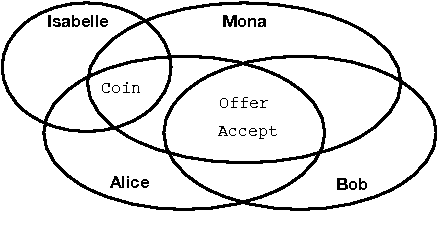
\includegraphics{figure/coin-transfer-visibility.pdf}
\end{center}
\vspace{-2ex}
\caption{Fact Visibility in Monitored Coin Transfer}
\label{f:CoinTransferVisibility}
\end{figure}

In many practical commercial workflows, it is either not desirable or not legal for all parties to be able to see all data in the system. In the coin transfer example from \S\ref{s:FactsWeights}, it is reasonable to expect that Alice would not want to reveal the total amount of coins she holds to Bob, nor the item she wishes to purchase (the Guitar) to Isabelle. Recall from \S\ref{s:Observation} that a party can see a fact when it is listed in either its \emph{by-authority} set or its \emph{obs-authority} set. We can express this as a simple predicate, where the functions \trm{auth-by} and \trm{auth-obs} retrieve the respective metadata from a fact value.
$$
\trm{sees}~ P~ F = |(\trm{auth-by}~F \cup \trm{auth-obs}~F) \cap \{P\}| \ge 0
$$
Applying this predicate to the initial facts from \S\ref{s:NowWithMetadata} we see that we already have the desired situation. The coin fact and its weight is visible to Alice (the giver), and Mona (the monitor), while the Offer and Accept facts only visible to Alice, Bob and Mona. Figure~\ref{f:CoinTransferVisibility} shows this in diagrammatic form.


% -----------------------------------------------------------------------------
% TODO: How does a confirming party know which other parties to ask for confirmations?
% It may see some in the facts revealed to it, but if a fact has been blinded it may not
% know it can ask the parties listed in that fact. We may want to add an extra field
% to the transaction listing the parties involved, which is separate from the facts
% themselves. This seems like a design variable where we might want the extra list,
% or not, and both answers are valid.

\subsection{Transactions and Validation}
\label{s:Transactions}
Maintaining fact privacy has implications for the underlying implementation. Assume that Alice, Bob, Mona and Isabelle all have their own computers in their own offices that each initially contain the subset of facts that each can see as per Figure~\ref{f:CoinTransferVisibility}. Assume that each party also has a copy of the transfer rule shown in Figure~\ref{f:CoinTransfer}. Now, suppose Alice decides that it is time to perform the transfer. On her own computer she executes the rule while recording the facts that have been consumed and the new facts that have been produced. She then builds a transaction data structure that records this information along with the cryptographic hash of the rule code, which we describe as so:

\begin{small}
\begin{code}
Transaction
 seq   = ... sequence number ...
 rule  = ... hash of code for transfer rule ...
 spent = [ Offer [id = '1234, terms = "To purchase a Guitar"
                  giver = !Alice, receiver = !Bob]
           by  {!Alice}            obs {!Mona, !Bob}
           use {'transfer}         num   1

         , Accept [id = '1234, accepter = !Bob]
           by  {!Bob}              obs {!Mona, !Alice}
           use {'transfer}         num 1

         , Coin   [issuer = !Isabelle, holder = !Alice]
           by  {!Isabelle, !Alice} obs {!Mona}
           use {'transfer}         num 1 ]

 new   = [ Coin   [issuer = !Isabelle, holder = !Bob]
           by  {!Isabelle, !Bob}   obs {!Mona}
           use {'transfer}         num 1 ]
\end{code}
\end{small}

This is the complete transaction that describes all inputs and outputs. Alice can send the complete transaction to Mona, which from Figure~\ref{f:CoinTransfer} is also entitled to see all the input and output facts. In contrast, Isabelle is not entitled to see the Offer fact as she is not listed as either an authorizer or an observer on it. Instead, Alice can compute a \emph{restricted view} of the transaction to send to Isabelle, which enables her to validate that Alice and Bob have authorized the coin facts to be moved, but does not reveal the Offer fact that contains the terms of the transfer.

Note that Alice herself is not listed in the meta-data of the produced coin fact, but will certainly know what this fact is because she is the one forming the transaction. In this case we say that Alice is an \emph{incidental observer} of this fact. Although Alice knows that this fact will be added to Isabelle, Bob, and Mona's view of the store, she should not add it to her own store. As Alice is not a \emph{formal observer} of the fact, she will be notified of transactions that spend this fact, so cannot be sure about its weight once her own transaction has been processed.

% Note that Bob is not listed in the metadata of the consumed coin fact, but will be able to infer its contents anyway because according to the transfer rule, the fields must match data in facts that he can see.


% -----------------------------------------------------------------------------
\subsection{Transaction Views}
Alice cannot sent the complete transaction from the previous section to Isabelle, as Isabelle is not entitled to see the contents of the Offer fact. However, Alice does wish Isabelle to know that transfer has taken place, and that Bob has agreed to it, because Isabelle is an authorizer of the Coin facts being moved. To achieve this Alice computes a \emph{restricted view} of the transaction for Isabelle, which consists of a blinded hash of the entire transaction, along with along with a version of the transaction structure where the facts that Isabelle is not entitled to see are replaced by blinded hashes of those facts. A \emph{blinded} hash is a regular cryptographic hash which has been combined with a salt value so that the source data cannot feasibly be recovered by brute force.

For the sake of presentation, lets abbreviate the factoids in the transaction from the previous section as just $d_1, d_2, d_3, d_4$, and write the complete transaction as the following tuple, where we use $h(X)$ to mean the hash of value $X$.
$$
 (seq,~ h(tx), [d_1, d_2, d_3], [d_4])
$$
The above tuple consists of the sequence number, hash of the code for the transaction rule (abbreviated $h(tx)$), a list of factoids being spent, and a list of factoids being created. To compute the blinded hash of the overall transaction we generate a random salt value for each of the factoids, $s_1 .. s_4$, and use it when hashing those factoids.
$$
\begin{array}{rl}
 \hspace{-2ex} h((seq,~ h(tx), [h(d_1, s_1), h(d_2, s_2), h(d_3, s_3)], [h(d_4, s_4)]))
\end{array}
$$
This value is a unique(ish) identifier for the transaction, assuming that the resulting hash values are long enough that we will not see a collision in practice. Now, as Isabelle is entitled to see the Coin facts but not the consumed Offer and Accept facts she receives a view containing the fact data and salt for the Coin facts, but only the blinded hash of the Offer and Accept facts.
$$
\trm{Isabelle:}~~(seq,~ h(tx), [h(d_1, s_1), h(d_2, s_2), (d_3, s_3)], [(d_4, s_4)])
$$
Similarly, Bob is entitled to see the Offer, Accept and produced Coin fact, but not the consumed Coin fact, so receives a corresponding view. Note that Bob can infer what the consumed coin fact will be anyway, but we leave the discussion of this to the next section.
$$
\trm{Bob:}~~(seq,~ h(tx), [(d_1, s_1), (d_2, s_2), h(d_3, s_3)], [(d_4, s_4)])
$$
Finally, Mona is entitled to see everything so she gets the same unblinded transaction that Alice has.
$$
\trm{Mona:}~~(seq,~ h(tx), [(d_1, s_1), (d_2, s_2), (d_3, s_3)], [(d_4, s_4)])
$$
All four parties, including Alice, are then able to use their transaction view to compute the same transaction identifier. Isabelle does not have the data for the Offer and Accept facts, but as she knows their hashes she can still form the hash of the overall transaction. Isabelle also cannot feasibly determine what the Offer and Accept facts originally were because the hashes of these facts have been salted by random numbers $s_1, s_2$ that she does not know. Isabelle \emph{can} determine that the $giver$ and $receiver$ fields of the Offer fact must have been @!Alice@ and @!Bob@ respectively as she knows the rule that the transaction was generated from, and the rule code reveals that these fields must match the corresponding fields in the Coin facts that she does see. Isabelle does not see that a Coin is being transferred @"To purchase on Guitar"@. That information is none of her business.


% -----------------------------------------------------------------------------
\subsection{Consensus}
Once Alice has sent the appropriate restricted transaction view to each party those parties can compare it against their own view of the current ledger state and confirm whether they believe it is valid. Isabelle is able to see the complete number of coins that are currently held by Alice, so Bob can ask Isabelle to confirm that her view of the transaction is valid, and hence enough coins were available for the transfer. In a practical workflow Isabelle would likely represent a commercial Bank, and Bob would trust Isabelle to answer truthfully when asked if enough coins are available for a currency transfer, even though he does not want the Bank to know that he is adding to his collection of guitars. Likewise, Isabelle can ask Bob to confirm that his view of the transaction is valid, and that he really did accept the transfer.

For a concrete implementation there are many ways to manage the transaction confirmation process. For a small number of parties, such as to manage commercial workflows between banks, it could be sufficient for each party to confirm the transaction directly with all others. This would require $O(n^2)$ confirmations in practice, but in the happy case the only information that needs to be exchanged is that the confirming party agrees with the transaction of the given hash code. For a greater number of parties, cryptographically signed confirmation messages could be propagated with a peer-to-peer protocol~\cite{El-Ansary2003:Broadcast}, or Byzantine Fault Tolerant (BFT) consensus protocol~\cite{Lamport1982:Byzantine, Ongaro2014:Consensus, Gilad2017:Algorand}



% Each transaction has a unique(ish) identifier consisting of the transaction hash, so each confirmation message is not a large amount of data.


% In hostile environment such as on the public internet the confirmations could be propagated via a , or one additionally resistant to Sybil attacks~\cite{}.

% Our programming model is not specific to any specific consensus mechanism, and different mechanisms are appropriate for different environments, so we do not seek to specify one here.


% -----------------------------------------------------------------------------
\subsection{Authorization Flow}
Note that in our system there is nothing preventing a party from adding a fact to the system which says ``I have a million dollars'', just with their own authority. As mentioned in \label{s:Authority} we allow parties to add arbitrary facts with their own authority, and delete fact that only authorized with their own authority. In the transaction structure of \S\ref{s:Transactions} this is achieved just by leaving the @rule@ field empty, as well as either the @spent@ or @new@ fields. The key property we need to manage is whether anyone else in the system should \emph{believe} those facts.

Recall that in the coin transfer example from \S\ref{s:Facts}, the coin facts always carry the authority of multiple parties, which is justified by the sequence of transactions that result in their production. The coin issuer (@Isabelle@ in the example) creates the initial coin facts, specifies the rules for using them, and signs the facts with their own authority. When the coins are transferred onwards the transactions recording the use of the transfer rule are also signed by the parties that propose them. Assuming most parties in the system are honest, invalid transactions will simply not be confirmed. Dishonest parties are free to corrupt their own databases by adding invalid transactions, but honest parties will not accept transactions that do not agree with their own view of the facts.

%  As with the consensus mechanism, our programming model does not specify a particular dispute mechanism, as different mechanisms are appropriate for different environments. In a commercial banking system it would be a rare occurrence for a party to actively propose an invalid transaction, so it may be appropriate to pause the system and investigate the issue manually. In a hostile internet environment it maybe instead be appropriate to blacklist the submitting party and not accept further transactions from them.

% -----------------------------------------------------------------------------
\subsection{Nested Transactions}
\label{s:NestedTransactions}
For the transaction described in \S\ref{s:Transactions}, the view to be given to Isabelle is constructed by blinding the @Offer@ and @Accept@ facts, as Isabelle is not an observer of these. Blinding these facts means that that Isabelle cannot use the information on the transaction to directly re-execute the rule and check the output. In an application where there is trusted monitor party such as Mona, this may not matter, as the monitor could be trusted to re-execute the transaction themselves and answer truthfully when asked if they believe it is valid. If we instead wish to allow Isabelle to validate the transaction output based on the input facts she can see, we can split the transfer rule into two parts: one part that checks that Alice and Bob agree on the offer, and another part concerning the actual coin transfer:

\begin{small}
\begin{code}
  rule  agreeOffer
  await Accept [id = ?i, accepter = ?a]            gain {a}
    and Offer  [id = i,  giver = g, receiver = ?a] gain {g}
  to
   say  Agreed [giver = g,   receiver = a]
    by  {g, a} obs {!Mona, !Isabelle}

  rule  doTransfer
  await Agreed [giver  = ?g, receiver = ?a] gain {g, a}
   and  Coin   [issuer = ?s, holder   = g]  gain {s, g}
  to
   say  Coin   [issuer = s,  holder   = a]
    by  {s, a} obs {!Mona, s, a}
\end{code}
\end{small}

With these two rule definitions Alice can build a nested transaction \CITE. For our purposes it is sufficient to represent a nested transaction as containing a list of sub-transactions as per the layout described in \S\ref{s:Transactions}, but with its own overall hash based identifier formed by combining the hashes of the sub-transactions. For the example above, the first sub-transaction will consume the @Accept@ and @Offer@ facts and produce and @Agreed@ fact with both Alice and Bob's authority. The second sub-transaction will immediately consume the @Agreed@ fact along with the @Coin@ fact, and produce a new @Coin@ fact. Importantly, both the created @Agreed@ fact in the first transaction, as well as the input @Coin@ fact are guaranteed to be visible to Isabelle, so she will be able to re-run the second sub-transaction and validate the output herself. Isabelle will still not be able to see the terms of the offer, but will be able to confirm with both Alice and Bob that they both agreed to it.

% The fact that some parties in a distributed system may not see all the components of a nested transaction is a common to most distributed database implementations.

% \TODO{Cite the XA distributed transaction model}.
% \TODO{Cite Corda Tearoffs}.
% \TODO{Cite Fabric private transactions} mentioned in DAML blog post.
% https://medium.com/daml-driven/keeping-smart-contracts-private-is-hard-unless-you-truly-understand-them-920b31d723e4

% TODO: contrast with DAML. In a DAML choice execution we always combine the authority
% of the contract instance with the controller of the choice. Both the signatories of the
% initial contract instance, and the controller can always see the full transaction, so
% we end up with partially blinded transactions like the first form of 'transfer'.


% -----------------------------------------------------------------------------
\subsection{Upgrade}
\label{s:Upgrade}
In practical information systems it is often necessary to upgrade data formats and business rules as requirements change over time. The fact that sets of rule names attached to each fact can be manipulated from the term language makes it easy to perform upgrades. For example, we can perform an upgrade of the business rules associated with @Coin@ fact using an upgrade rule such as:

\begin{small}
\begin{code}
  rule  upgrade
  await Coin [ issuer = ?s, holder = ?h ]  gain {s, h}
    and LetsUpgrade [ rules = ?rs ]     gain {!Operator}
    and YeahOk      [ party = s, rules = ?rs ] gain {s}
    and YeakOk      [ party = h, rules = ?rs ] gain {h}
   to
    say Coin [ issuer = s, holder = h ]
     by {s, h} use rs
\end{code}
\end{small}

Here, and @!Operator@ party adds an @UpgradePropose@ fact with a set of new rules that should be swapped in for the @use@ set of each coin. Once both the issuer and holder add facts that state they accept this upgrade the old coins can be consumed and new ones created that have the new @use@ set. The ability to upgrade the coins is specified by including the name of the upgrade rule in their original @use@ set (or not), but the new business rules can be specified after the initial coin facts have been generated.


% -----------------------------------------------------------------------------
\begin{figure}
\begin{center}
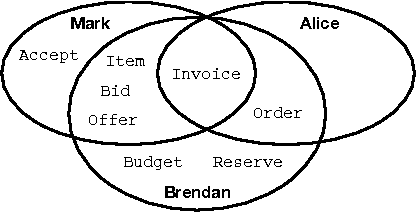
\includegraphics{figure/auction-visibility.pdf}
\end{center}
\vspace{-2ex}
\caption{Fact Visibility in Auction Example}
\label{f:AuctionVisibility}
\end{figure}


\subsection{Query}
\label{s:Query}
In our examples so far, each matching clause in a rule has always selected a single fact. In contrast, consider an auction workflow where we will need to rank offers by price, instead of just selecting any which matches. The fact visibility of such a workflow is depicted in Figure~\ref{f:AuctionVisibility}. Mark runs the auction market, Brendan is a broker, and Alice is a customer. The house rules are such that a customer (Alice) may not bid on items directly. Instead, the customer enlists a broker (Brendan) to which they provide an @Order@ describing the sort of @Item@ they wish to purchase, and their price limit. Naturally, the details of the @Order@ are private between the broker and customer, as the party running the auction house should not know the absolute maximum price a customer is willing to pay. During the auction, the market announces which items are for sale, including their lot number, description, and asking price. If anyone wishes to pay the asking price then the item is sold immediately. Bids may also be entered below the asking price, and the market will then communicate with the original owner of the item (not shown) about whether they are willing to sell at that lower price. The following rule shows how the broker can enter bids with the joint authority of themselves, as well as their customer:

\begin{small}
\begin{code}
fact Item  [lot: Nat, desc: Text, ask: Nat]
fact Order [buyer:  Party, desc: Text, limit: Nat]
fact Enter [broker: Party, lot: Nat, offer: Nat]
fact Bid  [broker: Party, buyer: Party, lot: Nat, offer: Nat]

  rule  bid
  await Item   [lot = ?n, desc = ?d, ask = ?a]
               select first a   consume none
    and Order  [buyer  = ?y, desc = d, limit = ?l] gain {y}
    and Enter  [broker = ?k, lot  = n, offer = ?o] gain {k}
         where o <= l && o <= a
  to
    say Bid    [buyer = y, broker = k, lot = n, offer = o]
     by {y, k} obs {!Mark}
\end{code}
\end{small}

In the first matching clause we have used @select first a@ to indicate that all matching @Item@ facts should be sorted by the asking price, and the first (cheapest) one selected. As the @Item@ fact is an announcement, rather than an asset to be ``spent'', we add @consume none@ to indicate the fact should not be consumed in the match. We have also added a @where@ clause to indicate that the offer entered by the broker must be no greater than the asking price for the item, or the limit of the customer. This allows the broker to use their own knowledge to try to get a better deal for the customer.

Finally, note that the transaction views generated from this rule that are given to Mark will have Alice's order fact blinded. In a practical implementation of an auction house workflow it may not be necessary for Mark to confirm the validity of each view in real time with Alice. Instead, after the auction is completed, if there is any dispute about about Brendan's involvement then he can provide the full transaction which includes Alice's signed order, as proof that he was acting in good faith.



